Over this chapter, the \textbf{space communication protocols} are going to be defined. That is, a set of rules are going to be established in order to achieve the actual node-to-node communication. Altough the scope of the chapter is limited to the space segment, this inital introduction on the protocol definition is usfeul for the ground segment.
Having said that, several factors constrain the design of this relation of rules:

\begin{itemize}
\renewcommand{\labelitemi}{\scriptsize$\blacksquare$} 
\item \textbf{Speed:} As it has already been mentioned, each node should be capable of handling at least \textbf{25} Mbit/s. Even though this doesn't mean that the design should be able to fit 25 Mbit/s of pure costumer data, it is still a strong requirement with many effects over the system. For example, some protocols are just too slow establishing the connection; those will be directly discarded.

\item \textbf{Reliability:} The protocols have to assure that the messages are going to arrive to their destination. In order to achieve this, a routing protocol has to be used as well.


\item \textbf{Security:} Messages are not just required to arrive to their destination but they also must be ordered and coherent when they reach the client. That is the reason why error control is taken into consideration very seriously along the design process.
\end{itemize}
In order to define the protocols, the standards of the Consultive Committee for Space Data Systems will be followed. The CCSDS define a set of standards that become part of ISO and enhance operatibility between different satellites. The protocols recommended by the CCSDS and the possible combinations between them are:
\begin{figure}[H]
\begin{center}
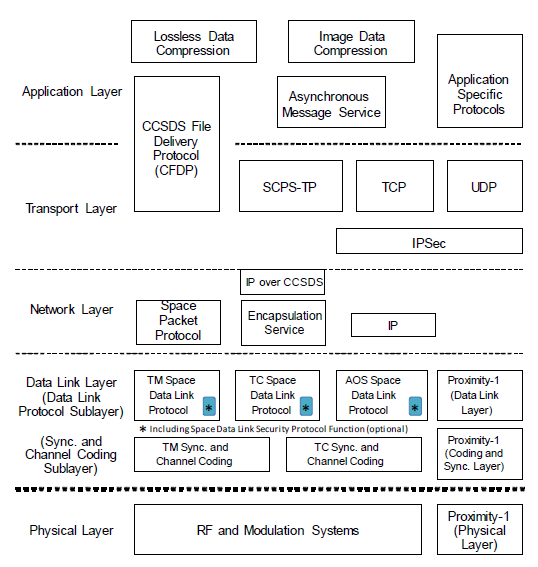
\includegraphics[scale=0.6]{SpaceSegment/Layer3/CCSDSprotocols.png}
\caption{Protocols recommended by the CCSDS, classified in their respective OSI layer. Extracted from \cite{CCSDSOverview}}
\end{center}
\end{figure}
\begin{figure}[H]
\begin{center}
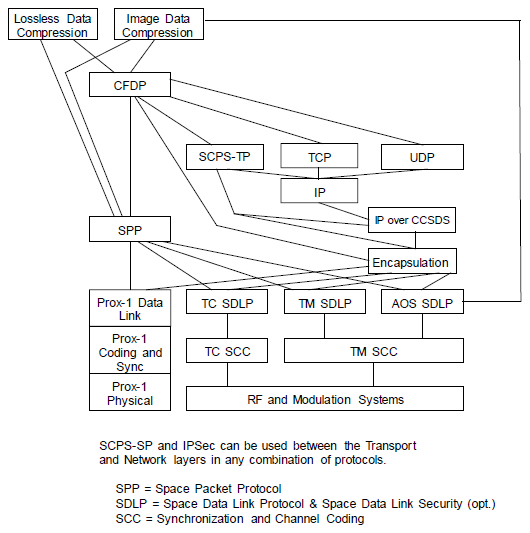
\includegraphics[scale=0.6]{SpaceSegment/Layer3/CCSDScombinations.png}
\caption{Possible combinations of the CCSDS recommended protocols. Extracted from \cite{CCSDSOverview}}
\end{center}
\end{figure}
As far as \textit{Astrea constellation} is concerned, the physical layer is already defined in detail in the \textbf{Satellite Desgin} part. Since the\textbf{ Data Link layer}, the \textbf{Network layer} and the \textbf{Transport/Session layer} are of vital importance for the communication to work, the aim of the next sections will be to define the protocol that the constellation will be using for each one of those layers.

The presentation and the application layer are more client oriented. In other words, if one client's satellite sends some data formatted with an unknown application protocol, \textit{Astrea} will not be affected in any way. What astrea will do is add to this stream of bits, some headers, in order for the message to arrive in time to its destination. This methodology is undoubtedly positive for \textit{Astrea} since the respobility of the application data will be solely for the customer.